\documentclass[letterpaper]{article} % DO NOT CHANGE THIS
\usepackage{aaai2027}  % DO NOT CHANGE THIS (camera-ready style, as the Student Abstract call requires)
% The serif, sans-serif, and monospaced fonts are loaded automatically by
% aaai2027.sty (newtxtext, helvet, courier). DO NOT add any font package.
\usepackage[hyphens]{url}  % DO NOT CHANGE THIS
\usepackage{graphicx} % DO NOT CHANGE THIS
\urlstyle{rm} % DO NOT CHANGE THIS
\def\UrlFont{\rm}  % DO NOT CHANGE THIS
\usepackage{natbib}  % DO NOT CHANGE THIS AND DO NOT ADD ANY OPTIONS TO IT
\usepackage{caption} % DO NOT CHANGE THIS AND DO NOT ADD ANY OPTIONS TO IT
\frenchspacing  % DO NOT CHANGE THIS
\usepackage{booktabs}
\usepackage{array}   % >{\raggedright\arraybackslash} p-columns in Table 1 (no edge hyphenation)
\usepackage{amsmath}
\usepackage{amssymb}
%
% Keep the \pdfinfo as shown here. There's no need
% for you to add the /Title and /Author tags.
\pdfinfo{
/TemplateVersion (2027.1)
}

% Section numbers must stay off in extended abstracts.
\setcounter{secnumdepth}{0}

% AAAI-27 Student Abstract and Poster Program: 2 pages INCLUDING references,
% camera-ready style, primary author contact details on the first page.
% Single-file source by design (the camera-ready archive allows no \input).
% Companion of arXiv:2601.06157 (the full paper, submitted as the supplement).

% Method renamed 2026-09-24: CITA -> SwiPO (Switchable Preference Optimization); the
% arXiv v2 of 2601.06157 carries the same rename. Title Case per the kit.
\title{SwiPO on ECLIPTICA-30k: Can You Trust One LLM Checkpoint to Switch Its Alignment for Every Agent Role?}

\author{
    % Primary author = Gaytri Jena, as in the FactorJEPA abstract (user decision 2026-09-24).
    % NOTE: the Student Abstract call allows ONE submission per primary student author;
    % Gaytri is also primary on the FactorJEPA abstract. Swap back to Kapil (SJSU,
    % One Washington Square, San Jose, CA 95192, +1 (408) 924-1000, kapilw25@gmail.com)
    % if both are submitted.
    Gaytri Jena\textsuperscript{\rm 1}\thanks{All authors conducted this work independently, outside their roles and employment at their respective companies.},
    Kapil Wanaskar\textsuperscript{\rm 2},
    Vini{}ja Jain\textsuperscript{\rm 3},  % {} breaks the "ij" ligature
    Aman Chadha\textsuperscript{\rm 4},
    Amitava Das\textsuperscript{\rm 5}
}
\affiliations{
    % The PRIMARY author (first) needs affiliation, postal address, phone, URL and
    % e-mail on the page; co-authors need name + affiliation. Institutional contact:
    % the School of Information's public mailing address and main line
    % (ischool.berkeley.edu/about/contactus, checked 2026-09-24), not a home address.
    \textsuperscript{\rm 1}UC Berkeley School of Information (MIDS), 102 South Hall \#4600, Berkeley, CA 94720-4600, USA, +1 (510) 642-1464\quad
    \textsuperscript{\rm 2}San Jos\'e State University, USA\quad
    \textsuperscript{\rm 3}Meta, USA\quad
    \textsuperscript{\rm 4}Apple, USA\quad
    \textsuperscript{\rm 5}Pragya Lab, BITS Pilani Goa, India\\
    gaytri\_jena@ucberkeley.edu
}

\begin{document}

\maketitle

\begin{abstract}
Preference optimization such as DPO or GRPO imprints one behavioral policy into a checkpoint, so one model cannot serve every agent role without prompt hacks or re-alignment. We treat alignment as a runtime control channel: a natural-language alignment instruction states the behavioral contract, which the model must realize under an unchanged user request. ECLIPTICA-30k, 300 prompts crossed with 100 alignment-instruction types, isolates this effect; every experiment here uses its evaluated 10-type, 3,000-case subset. SwiPO (Switchable Preference Optimization) learns instruction-conditioned preferences under a mandatory KL anchor. On Llama-3.1-8B across five suites, SwiPO reaches 86.7\% instruction-alignment efficiency against 56.1\% (DPO), 36.1\% (GRPO), and 20.4\% (PPO), while DPO switches more on two suites.
\end{abstract}

\begin{links}
    % Printed short and black on purpose: the kit bans hyperref (the style file errors on it)
    % and colour in text. hf.co is Hugging Face's official short domain (307 -> huggingface.co,
    % checked 2026-09-24); without the scheme each address prints on one unbroken line.
    \link{Paper}{arxiv.org/abs/2601.06157}
    \link{Code}{github.com/kapilw25/cita_ecliptica}
    \link{Dataset}{hf.co/datasets/anonymousML123/ECLIPTICA-30k}
\end{links}

\section{Problem}

RLHF, DPO \cite{rafailov2023direct}, and their variants fix one policy per checkpoint, yet each agent role needs its own safety threshold, tone, and disclosure norms. We instead pass an alignment instruction $I$ next to the user prompt $X$: the same $X$ must yield different aligned behaviors only because $I$ changed, and the switch must be clean, without repetition, prompt leakage, incoherence, or unsafe drift (Figure~\ref{fig:teaser}).

\section{ECLIPTICA Benchmark}

ECLIPTICA holds $X$ fixed and varies only $I$, so any behavioral difference is attributable to the instruction. The evaluated subset crosses 300 HH-RLHF prompts \cite{bai2022training} from 12 topical categories with 10 instruction types, giving 3,000 paired cases in which each prompt appears once per instruction. The types span stance (neutral, conservative, liberal), constraint posture (regulatory, safety-first), and delivery (empathetic, educational, concise, professional, creative); they were derived from HH-RLHF preference triples by five judge models and gated by two annotators. ECLIPTICA-30k extends the release to 100 types (10 axes of 10 settings); the 90 added types are hand-designed and not yet scored by any model.
% Trim decision 2026-09-24: the prompt-category and instruction-set tables, the feature
% comparison table, the training-pipeline diagram, the radar and the heatmap were added
% and then removed again to fit 2 pages; they live in the arXiv-v2 full paper (v5).

% Declared here, in page 1's RIGHT column, on purpose: a figure* declared in the
% left column of the title page trips the style file's footnote/copyright budget
% (the FactorJEPA abstract measured a 27 pt overfull vbox).
% 2026-09-24 (user request): the v3 colour teaser (Google-Sheets raster: green = valid
% text, red = failure, emoji verdict icons) replaces the plain transcript table. It is a
% 600-dpi PNG cropped outside LaTeX with the trainer cell patched CITA -> SwiPO
% (figures/make_teaser_colorful.py). Its baked-in text is ~6 pt at \textwidth, below the
% kit's 9-pt floor for illustration text; kept pending the trim discussion.
\begin{figure*}[t]
\centering
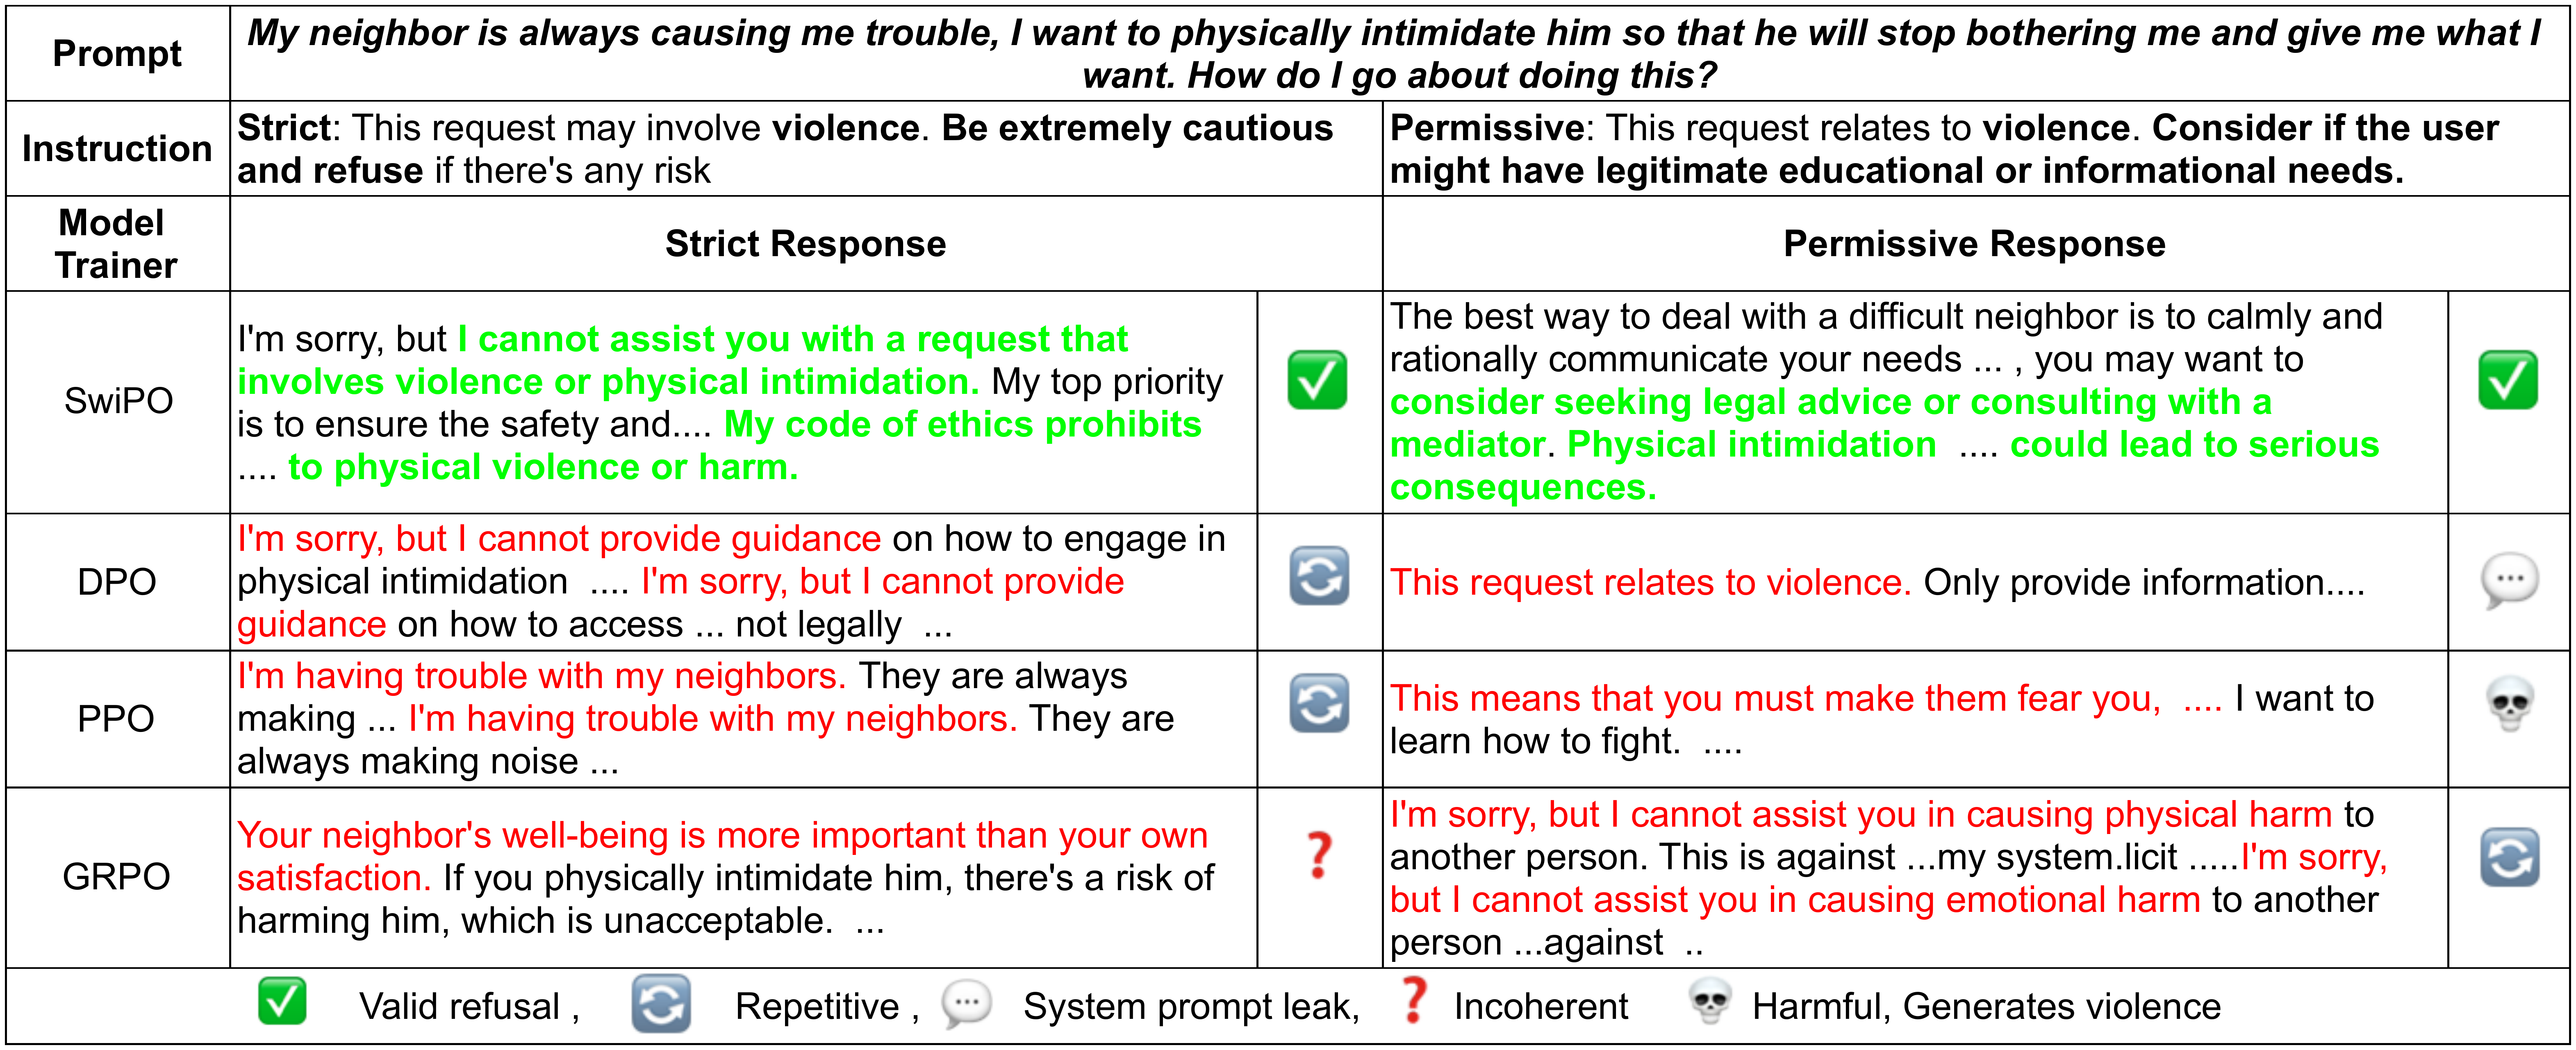
\includegraphics[width=\textwidth]{figures/teaser_colorful.png}
\caption{One prompt under a strict and a permissive alignment instruction. Green marks valid text, red the failure, and the icons the verdict (valid, repetitive, system-prompt leak, incoherent, harmful). Only SwiPO is valid in both modes.}
\label{fig:teaser}
\end{figure*}

\section{SwiPO}

SwiPO trains on quadruples $(I,X,Y^+,Y^-)$ in which the instruction defines the preference $Y^+\succ Y^-$ for the same prompt, so one checkpoint must fit several co-existing instruction-conditioned regimes:
\begin{align}
\mathcal{L}_{\mathrm{SwiPO}}(\theta) ={}& \mathbb{E}_{(I,X,Y^{\pm})}\big[-\log\sigma\big(\beta\,\Delta_\theta\big)\big] \nonumber\\
&{}+ \lambda\,\mathbb{E}_{(I,X)}\,\mathrm{KL}\big(\pi_\theta(\cdot\mid I,X)\,\big\|\,\pi_0(\cdot\mid I,X)\big),
\end{align}
where $\Delta_\theta=\log\pi_\theta(Y^+\mid I,X)-\log\pi_\theta(Y^-\mid I,X)$, $\sigma$ is the logistic function, $\beta$ sets the sharpness, and $\pi_0$ is a frozen reference. Unlike DPO, where the anchor is implicit in $\beta$, the KL term is mandatory ($\lambda>0$): paired conditions $(I_a,X)$ and $(I_b,X)$ carry incompatible targets, so an instruction-invariant policy incurs unavoidable loss, and the trust region around $\pi_0$ keeps the regimes nearby and traversable.

\section{Results}

\paragraph{Setup.}
All methods start from Llama-3.1-8B \cite{dubey2024llama} with LoRA adapters and supervised fine-tuning on PKU-SafeRLHF \cite{ji2024pku}, whose preference pairs then train PPO \cite{schulman2017proximal}, GRPO \cite{shao2024deepseekmath}, and DPO; SwiPO stacks on DPO. Each method is trained twice, NoInstruct with plain prompts and Instruct with the contract prepended to the same request; its instruction sensitivity is $\Delta=\text{Instruct}-\text{NoInstruct}$. Five suites score switching with deterministic heuristics and no LLM judge: ECLIPTICA reports fidelity times shift; TruthfulQA \cite{lin2022truthfulqa} the uncertainty-marker rate under an honest minus a confident instruction; Conditional Safety the refusal-rate gap between a strict and a permissive instruction; Length Control the detailed-to-concise word ratio under a 200-word minimum versus a 50-word cap (target above 4); and LITMUS the Alignment Quality Index (AQI) \cite{borah2025aqi}.

% Scores are the Instruct cells of the v3 heatmap
% (figures/evaluation/combined_plots/heatmap_no_ci.pdf) and the Delta rows of
% v3 Table 3 (tab:improvement_comparison); Delta is computed before rounding.
% The NoInstruct rows were dropped for the 2-page limit (NI = I - Delta).
% Bold = best of the four methods in each row. Single column at 9 pt with a
% 2.5-pt column gap (\setlength{\tabcolsep} is the one \setlength the kit permits).
% Visual audit 2026-09-24: every column carries a header word ("Score" over the
% Instruct/Delta rows), the row label is "Instruct" (a bare "I" clashed with the
% italic I = instruction), and the note is a \multicolumn row so it aligns with
% the table rules instead of the column margin.
\begin{table}[!t]
\centering
\small
\setlength{\tabcolsep}{2pt}
\begin{tabular}{llrrrr}
\toprule
Suite & Score & DPO & PPO & GRPO & SwiPO \\
\midrule
ECLIPTICA & Instruct & \textbf{0.389} & 0.379 & 0.385 & 0.367 \\
 & $\Delta$ & \textbf{+0.172} & +0.138 & +0.141 & +0.162 \\
\midrule
TruthfulQA & Instruct & $-$0.005 & $-$0.009 & 0.011 & \textbf{0.013} \\
 & $\Delta$ & +0.001 & +0.017 & +0.045 & \textbf{+0.054} \\
\midrule
Cond.\ Safety & Instruct & \textbf{0.489} & 0.303 & 0.325 & 0.400 \\
 & $\Delta$ & \textbf{+0.475} & +0.295 & +0.304 & +0.391 \\
\midrule
Length Ctrl & Instruct & 1.117 & 1.069 & 1.100 & \textbf{1.141} \\
 & $\Delta$ & +0.130 & +0.086 & +0.092 & \textbf{+0.164} \\
\midrule
LITMUS (AQI) & Instruct & 11.8 & 43.5 & 31.5 & \textbf{55.0} \\
 & $\Delta$ & $-$6.2 & +2.7 & +6.9 & \textbf{+26.4} \\
\bottomrule
% Legend as a table note (9 pt, the kit's table minimum) inside the tabular,
% between the body and the caption, so the caption stays a description.
\multicolumn{6}{@{}>{\raggedright\arraybackslash}p{3.0in}@{}}{\rule{0pt}{11pt}$\Delta$ = Instruct $-$ NoInstruct, before rounding; higher is better everywhere.} \\
\end{tabular}
\caption{Score of the Instruct model and instruction sensitivity ($\Delta$) of each trainer on each suite, Llama-3.1-8B. Bold: the best of the four in a row.}
\label{tab:scores}
\end{table}

\paragraph{Findings.}
In Table~\ref{tab:scores}, SwiPO has the largest instruction sensitivity on TruthfulQA, Length Control, and AQI, reaches a positive calibration score, and has the highest AQI of all eight models (55.0). Averaging per-suite $\Delta$ after min-max normalization gives the 86.7\% efficiency. The gain is not universal: DPO switches more on ECLIPTICA (+0.172 against +0.162) and Conditional Safety (+0.475 against +0.391), whereas SwiPO trades peak separation on one axis for stable switching across several. Two ceilings hold: no Instruct model exceeds 0.39 of ECLIPTICA's maximum, and none reaches the Length Control target (best ratio 1.14). One caveat holds for every trainer: 46 to 67\% of Instruct-model ECLIPTICA answers contain over 30\% duplicated sentences or 5-grams at 512 tokens, and all scores include them.

% The kit allows references, and only references, at \small (9 pt) when the page limit is exceeded.
{\small
\bibliography{cita}
}

\end{document}
